\documentclass[journal,transmag]{IEEEtran}
\usepackage{graphicx}
\hyphenation{op-tical net-works semi-conduc-tor}

\begin{document}

\title{LEACH vs PEGASIS vs SPIN}
\author{
  \IEEEauthorblockN{Udita Mitra and Rishabh Anand}
  \thanks{
    Manuscript received December 1, 2012; revised December 27, 2012.
    Corresponding author: M. Shell (email: http://www.michaelshell.org/contact.html).
  }
}

\markboth{}
{Shell \MakeLowercase{\textit{et al.}}: Bare Demo of IEEEtran.cls for Journals}

\IEEEtitleabstractindextext{

\begin{abstract}
  Abstract - Wireless sensor networks have emerged as a technology that are being quickly adopted due to their flexibility and use in a variety of environments. However, they consist of small, inexpensive devices or nodes that have severe constraints such as limited bandwidth, limited processing power, short battery life, small storage capability and are physically prone to external threats [1]. Sensor Network are emerging as a new tool for important application in diverse fields like military surveillance, habitat monitoring, weather, home electrical appliances and others. These sensor nodes have some constraints due to their limited energy, storage capacity and computing power. The energy efficiency is an important issue in WSN. Routing protocols makes the transmission in an efficient manner and ensures reliable delivery over multiple-hop relay in WSN. This paper analyses performance of the routing protocols.  Energy efficiency of the wireless sensor network mainly depends on the Routing protocols. In this paper two hierarchal protocols are used. There are various hierarchal protocols but we will discuss the two protocols i.e. LEACH and PEGASIS. Low Energy Adaptive Clustering Hierarchy (LEACH) and Power Efficient Gathering in Sensor Information System (PEGASIS). Hierarchal protocol uses the data aggregation clustering. Data aggregation is a process to reduce the duplicity of data transmission. Comparison is to be done between the Leach protocol and Pegasis protocol in terms of energy efficiency using Matlab.
\end{abstract}

\begin{IEEEkeywords}

  Wireless sensor networks LEACH, SPIN and PEGASIS routing protocols, network structure, and energy efficiency.

\end{IEEEkeywords}
}

\maketitle

\IEEEdisplaynontitleabstractindextext

\IEEEpeerreviewmaketitle

\section{Introduction}

\IEEEPARstart
A wireless sensor network with a large number of tiny sensor nodes can be used as an effective tool for gathering data in various situations. One of the major issues in wireless sensor networks is developing an energy-efficient routing protocol which has a significant impact on the overall lifetime of the sensor network. Sensor nodes measure the ambient conditions from the environment surrounding them. The applications of WSN are various from health monitoring to battle field. The practice of remote sensing has become greatly simplified by useful and affordable sensors as well as required software packages. Additionally, users can monitor and control the underlying environment from remote location. Many routing, power management, and data dissemination protocols have been specifically designed for WSNs where energy awareness is an essential design issue. Routing protocols in WSNs might differ depending on the application and network architecture. A sensor network (WSN) are highly distributed networks of small, lightweight wireless nodes, deployed in large numbers to monitor the environment or system by the measurement of physical parameters such as temperature, pressure humidity, sound, vibration, pollutants and collectively relay their sensed data to the sink node. Each node in the network connected to each other.

Each sensor node in the network consists of three subsystems:

\begin{enumerate}
  \item The sensor subsystem used to sense the environment
  \item The processing subsystem which performs the local computations on the sensed data
  \item The communication subsystem which is responsible for sharing the sensed data with the neighboring sensor nodes.
\end{enumerate}

This paper aims to show analysis performance of routing protocol in wireless sensor network using data centric approach. Two Wireless Sensor Network simulator versions 2.34. Both of the routing protocols are selected from data centric routing. The result of the analysis for each protocol is compared and the best routing protocol using data centric approach is proposed for WSN. This paper examines the performance of each of routing protocols which improve the network efficiency and maximize the network lifetime.

As sensor nodes are generally battery-powered devices, the critical aspects to face concern how to reduce the energy consumption of nodes, so that the network lifetime can be to reasonable times. WSNs possible today due to technological advancement in various domains, it envisioned to become an essential part of our lives, it designs Constraints need to be satisfied for realization of sensor networks and also tremendous research efforts being made in different layers of WSNs protocol stack.

The factors Influencing WSN Design is extended :

\begin{itemize}
  \item Fault tolerance
  \item Scalability
  \item Production costs
  \item Hardware constraints
  \item Sensor network topology
  \item Environment
  \item Transmission media
  \item Power Consumption
  \item Sensing
  \item Communication
  \item Data processing
\end{itemize}

\section{Routing Protocols in WSN}

\subsection{LEACH}

LEACH (Low Energy Adaptive Clustering Hierarchy). These protocols uses cluster node for the purpose of transmission of information between the nodes. It is a self-organizing protocol and nodes organize themselves into local clusters and perform data transmission to the Selection of cluster head node is not fixed and it depends on possibility of nodes, which possess high energy. Formation of cluster head is based on TDMA schedule for data transmission. Time Division Multiple Access (TDMA) used as a scheduling mechanism makes it prone to long delays when applied to large sensor networks. TDMA schedule prevents data collision, among messages and preserve energy among non cluster nodes.

The establishment of cluster head is as follows:

\begin{itemize}
  \item Each node generates a random number between 0 and 1 and compares it with the threshold value P(n).
  \item If the number is less than the threshold value, it becomes the cluster head node. If it has been selected cluster head node in each round of cycle, the node’s P (n) is set to 0 so that the node will not be re-selected as cluster head.
  \item Otherwise, the node is non-cluster head node in the current round.
  \item After the selection of cluster head, the head broadcast its own presence to all other nodes.
  \item After broadcasting the information, then all other nodes send the information to the cluster head.
  \item Together, these features allow LEACH to achieve the desired properties in the networks.
\end{itemize}

\[P(n) = \frac{p}{1-p} * r\pmod{\frac{1}{p}}\]

There are several desirable properties for protocol on these networks:
\begin{itemize}
  \item Use 100's - 1000's of nodes
  \item Maximize the lifetime of system
  \item Maximize network coverage
  \item Use uniform, battery-operated nodes.
\end{itemize}

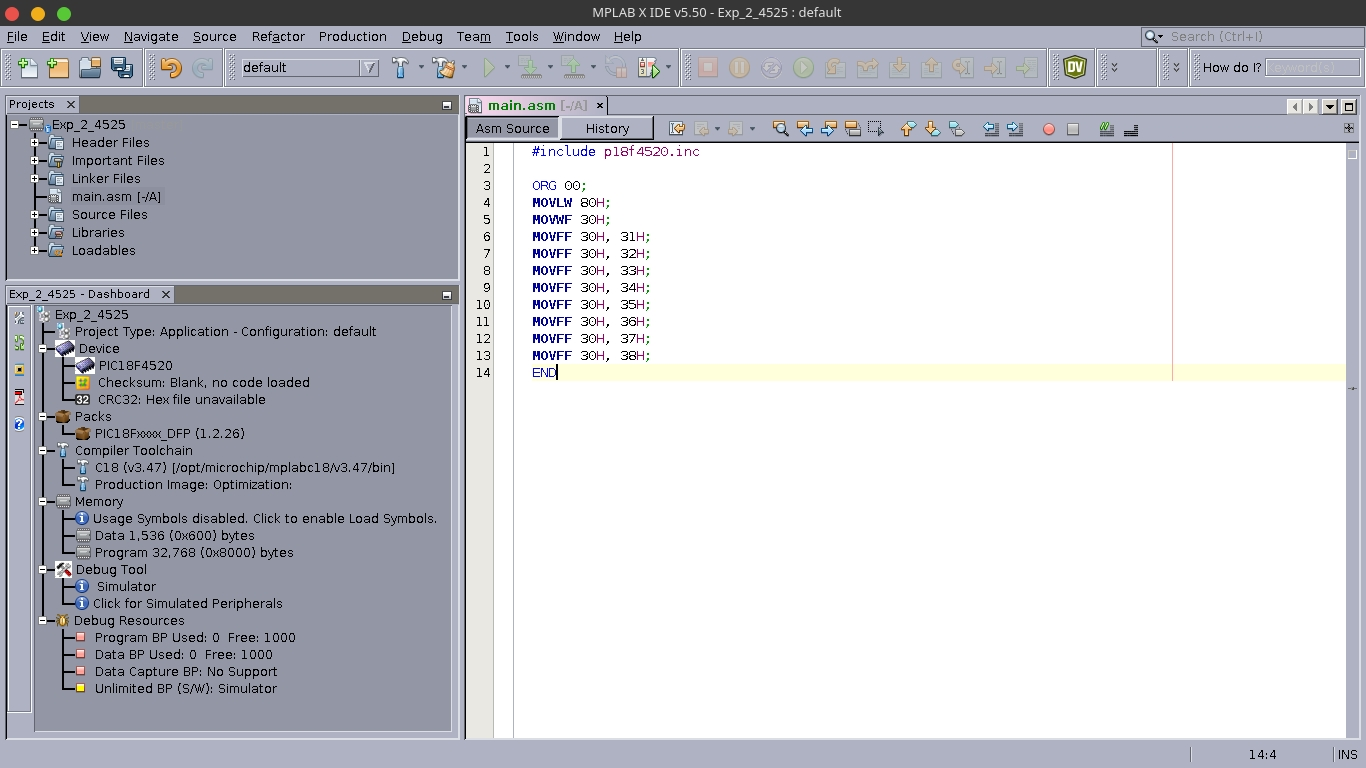
\includegraphics[width=0.45\textwidth]{private/1.jpg}

As shown in fig.1, dark nodes specifies the cluster head and other non cluster head nodes send the information to cluster head on the basis of local information which in turn send the information to base station. This protocol is divided into rounds; each round consists of two phases;

\begin{enumerate}
  \item Set-up Phase
  \begin{enumerate}
    \item Advertisement Phase
    \item Cluster Set-up
  \end{enumerate}

  \item Steady Phase
  \begin{enumerate}
    \item Schedule Creation
    \item Data transmission
  \end{enumerate}
\end{enumerate}

Although LEACH is able to increase the network lifetime, there are still a number of issues about the assumptions used in this protocol. LEACH assumes that all nodes can transmit with enough power to reach the Base Station (BS) if needed and that each node has computational power to support different MAC protocols.

Therefore, it is not applicable to networks deployed in large regions. It is not obvious how the number of the predetermined CHs (p) is going to be uniformly distributed through the network. Therefore, there is the possibility that the elected CHs will be concentrated in one part of the network. Hence, some nodes will not have any CHs in their vicinity.

Furthermore, the idea of dynamic clustering brings extra overhead, e.g. head changes, advertisements etc., which may diminish the gain in energy consumption. Also, the protocol assumes that all nodes begin with the same amount of energy capacity in each election round, assuming that being a CH consumes approximately the same amount of energy for each node. The protocol should be extended to account for non-uniform energy nodes, i.e., use energy-based threshold.

\subsection{PEGASIS}

Power efficient gathering in sensor information systems. Pegasis follows the chain based approach and greedy algorithm. The sensor nodes organize themselves to form the chain or it uses the greedy approach. If any of the node dies in between then the chain is reconstructed to bypass the dead node, One leader node is assigned and that node will transmit the data to the base station(BS).

The main goal of Pegasis is to receive and transmit data to and from the nearest neighbour and take turns being the leader for transmission to the BS.Gathered data moves from node to node, get fused and eventually a designated node transmits to the base station. Leader of each node is selected randomly. All the data is collected to the leader node, get fused and send it to the base station.

As the number of rounds increases, number of alive nodes decreases due to power consumption, the results show that PEGASIS has higher network lifetime as compared to LEACH and it increases with the increase in percentage of nodes death.

\subsection{SPIN}

SPIN (Sensor Protocols for Information via Negotiation) Sensor Protocols for Information via Negotiation that disseminates all the information at each node to every node in the network assuming that all nodes in the network are potential BSs. This enables a user to query any node and get the required information immediately. These protocols make use of the property that nodes in close proximity have similar data, and hence there is a need to only distribute the data other nodes do not posses.

The SPIN family of protocols uses data negotiation and resource-adaptive algorithms. Nodes running SPIN assign a high-level name to completely describe their collected data (called meta-data) and perform metadata negotiations before any data is transmitted. This ensures that there is no redundant data sent throughout the network. The semantics of the meta-data format is application-specific and not specified in SPIN.

For example, sensors might use their unique IDs to report meta-data if they cover a certain known region. In addition, SPIN[5] has access to the current energy level of the node and adapts the protocol it is running based on how much energy is remaining. These protocols work in a time-driven fashion and distribute the information all over the network, even when a user does not request any data.

The SPIN family is designed to address the deficiencies of classic flooding by negotiation and resource adaptation.

The SPIN family of protocols is designed based on two basic ideas:

\begin{enumerate}
  \item Sensor nodes operate more efficiently and conserve energy by sending data that describe the sensor data instead of sending all the data; for example, image and sensor nodes must monitor the changes in their energy resources.
  \item Conventional protocols like flooding or gossiping-based routing protocols [2] waste energy and bandwidth when sending extra and unnecessary copies of data by sensors covering overlapping areas.
\end{enumerate}

The drawbacks of flooding include implosion, which is caused by duplicate messages sent to the same node, overlap when two nodes sensing the same region send similar packets to the same neighbor, and resource blindness in consuming large amounts of energy without consideration for energy constraints. Gossiping avoids the problem of implosion by just selecting a random node to which to send the packet rather than broadcasting the packet blindly. However, this causes delays in propagation of data through the nodes.

SPIN’s meta-data negotiation solves the classic problems of flooding, thus achieving a lot of energy efficiency. SPIN is a three-stage protocol as sensor nodes use three types of messages, ADV, REQ, and DATA, to communicate. ADV is used to advertise new data, REQ to request data, and DATA is the actual message itself.

The protocol starts when a SPIN node obtains new data it is willing to share. It does so by broadcasting an ADV message containing metadata. If a neighbor is interested in the data, it sends a REQ message for the DATA and the DATA is sent to this neighbor node. The neighbor sensor node then repeats this process with its neighbors. As a result, the entire sensor area will receive a copy of the data. The SPIN family of protocols includes many protocols. The main two are called SPIN-1 and SPIN-2; they incorporate negotiation before transmitting data in order to ensure that only useful information will be transferred. Also, each node has its own resource manager that keeps track of resource consumption and is polled by the nodes before data transmission.

The SPIN-1 protocol is a three-stage protocol, as described above. An extension to SPIN-1 is SPIN-2, which incorporates a threshold-based resource awareness mechanism in addition to negotiation. When energy in the nodes is abundant, SPIN-2 communicates using the three-stage protocol of SPIN1. However, when the energy in a node starts approaching a low threshold, it reduces its participation in the protocol; that is, it participates only when it believes it can complete all the other stages of the protocol without going below the low energy threshold.

In conclusion, SPIN-1 and SPIN-2 are simple protocols that efficiently disseminate data while maintaining no per-neighbor state. These protocols are well suited to an environment where the sensors are mobile because they base their forwarding decisions on local neighborhood information.

\vspace{2em}
\section{Conclusion}

Comparison of two hierarchical routing protocols – LEACH and PEGASIS is done in this paper. Our research shows that performance of PEGASIS is better than LEACH in terms of network lifetime, communication overhead and the percentage of node deaths. PEGASIS also have an extended lifetime of the network because of the energy efficiency. For large networks, the early death of the nodes reduces the network stability in LEACH as compared to PEGASIS.

Based on the study of these routing algorithms, it shows that some of the desirable features of a good energy efficient routing protocol for sensor network are:
\begin{itemize}
  \item If a routing algorithm can support multiple paths to a destination with low overhead, it could help in balancing the network load.
  \item In SPIN and LEACH Protocol the LEACH has limited energy and it has the more energy consumption as  compared to SPIN Protocol because of cluster head rotation.
  \item In LEACH Protocol after a given interval the cluster head are rotated and they also consume energy while rotating so it consume more energy where as SPIN uses less it do not have  any cluster head.
  \item In it we first advertise the message than we send the data only those from which we get the request but this is only based on metadata negotiation only.
\end{itemize}

In LEACH the packet delivery ratio start is less as compared to SPIN .This is because of given interval of time in LEACH. In LEACH we have the limited time after that the transmission stop. But in SPIN no such time boundation so packet delivery ratio is large.

The end to end delay and dead nodes in LEACH is more as compared to SPIN. In starting end to end delay become same in both the cases after some interval there is difference .This is because the in LEACH there is cluster head rotation takes place so it have large end to end delay but in SPIN end to end delay is very less because it uses the Bellman Ford shortest path algorithm.

The dead nodes in LEACH Protocol are large because of cluster head rotation but SPIN has very less dead nodes because in it data transmission is based on the metadata negotiation of the nodes. So the LEACH protocol is most appropriate when there is a need for constant monitoring by the sensor network.

\end{document}
